%MPEG1/2 layers I/II encoder using a RISC-V processor and hardware accelerators
 
%This section, or section group, should explain in detail the problem this work is trying to solve and why it is essential. More sections containing background or state-of-the-art descriptions may be added if that improves the explanation.
%Describe the existing attempts at solving the problem and their limitations. One must perform a bibliography search, identify the principal works on this topic, and reference them in this document. An example citation is given in this sentence [1].

\subsection{MPEG-1/2 Layers I/II}

The Moving Picture Experts Group (MPEG) is a working group that sets standards for media coding, established by the International Organization for Standardization (ISO)~\cite{iso} and the International Electrotechnical Commission (IEC)~\cite{iec}. Thus, the MPEG standard is a set of specifications for audio and video compression, containing two variations (among others), MPEG-1 and MPEG-2. Both variations cover audio and video, but since this work is focused on audio, the relevant standards are MPEG-1 Audio and MPEG-2 Audio.
%is a working group of ISO/IEC with the mission to develop standards for coded representation of digital audio and video and related data.

The MPEG-1 Audio, defined by ISO/IEC 11172-3~\cite{11172} (explained in the next section), standardizes the information that an audio encoder must produce to write a bitstream conformant with the standard requirements. Moreover, it standardizes how an audio decoder has to parse, decompress, and resynthesize the information to reconstruct the original audio stream.

This standard performs perceptual audio coding, which does not attempt to retain the input signal exactly after encoding and decoding. Instead, it ensures that the output signal sounds the same to a human listener. %, by eliminating the parts of the input signal that are irrelevant to the human ear 
More precisely, an MPEG-1 audio encoder transforms the sound signal into the frequency domain, eliminates the frequency components that are masked by stronger frequency components, and packages the analyzed signal into a compressed audio bitstream.

%working principle
Focusing on the encoding process, the primary psychoacoustic effect is called "auditory masking", where parts of a signal are not audible due to the function of the human auditory system. For example, if there is a sound that consists mainly of one frequency, all other sounds that consist of a close frequency but are much quieter will not be heard. \\
%where exploiting the limitations of perception and removal of irrelevance is key to achieving a significant reduction in bitrate while preserving subjective audio quality.
Considering this, the parts of the signal that are masked are commonly called irrelevant, as opposed to the redundant parts that are removed. % by a lossless coding operation 
To eliminate this irrelevancy, the encoder contains a \textbf{psychoacoustic model} which analyzes the input signals within consecutive time blocks and determines, for each block, the spectral components of the input audio signal (by applying a \textbf{frequency transform}). Then, it models the masking properties of the human auditory system, and estimates the noise level for each frequency band, usually called "threshold of masking". 
In parallel, the input signal is fed through a time-to-frequency mapping, resulting in spectrum components for subsequent coding. \\
Finally, in the \textbf{quantization and coding} stage, the encoder tries to allocate the available number of data bits, meeting both the bitrate and masking requirements ("threshold of masking"). The information on how the bits are distributed over the spectrum is contained in the bitstream as side information.

%layers
The MPEG-1 standardizes three different coding schemes, namely Layer I, Layer II, and Layer III, with the first two layers being the relevant ones in this work.
Layer I has the lowest complexity and is specifically suitable for applications where the encoder complexity plays an important role.
Layer II requires a more complex encoder and decoder, being directed towards one-to-many applications, i.e. one encoder serves many decoders. 

Compared to Layer I, Layer II can remove more of the signal redundancy and apply the psychoacoustic threshold more efficiently.
%bitstream
In Layer II, the digitized audio signal is divided into blocks of 1152 samples, with each block being encoded within one MPEG-1 audio frame.
Therefore, an MPEG-1 audio stream consists of consecutive audio frames, each one containing a header and the encoded data. The header contains general information, such as MPEG Layer, sampling frequency, number of channels, etc. Although most of this information may be the same for all frames, MPEG decided to give each audio frame a header to simplify synchronization and bitstream editing.

%MPEG-2
All the previous information describes one variation of MPEG, MPEG-1 Audio. This variation represents the first phase of dealing with mono and two-channel stereo sound coding, at sampling frequencies commonly used for high-quality audio (48, 44.1, and 32 kHz).\\
In addition, there is a second variation, MPEG-2 Audio, which includes three main points.
The first point is the extension of MPEG-1 to lower sampling frequencies (16 kHz, 22.05 kHz, and 24 kHz), providing better sound quality at very low bit rates.
The second point is the backward-compatible (BC) extension of MPEG-1 to multichannel sound, supporting up to 5 full bandwidth channels plus one low-frequency enhancement channel. The MPEG-2 BC stream adheres to the structure of an MPEG-1 bitstream, meaning that an MPEG-2 BC stream can be read and interpreted by an MPEG-1 audio decoder.
The third and last point is a new coding scheme called Advanced Audio Coding (AAC), which is more efficient and presents higher quality.
 
%applications
Today, the MPEG-1 Audio standard is the most widely compatible lossy audio format in the world, thanks to technical merits and excellent audio quality performance.
Within the professional and consumer market, four fields of applications can be identified, namely broadcasting, storage, multimedia, and telecommunication. %This variety of applications is possible because of the wide range of bitrates and the numerous configurations allowed in MPEG-1. \\
% What is the work? motivation?

\subsection{MPEG-1/2 Layers I/II IP cores}

Knowing the wide range of customers that need digital audio, belonging to all industries, this work proposes developing an IP core to encode MPEG-1/2 Layer II, using a RISC-V processor and hardware accelerators.
 
An intellectual property core (IP core) consists of a block of logic or data that is used in a semiconductor chip when making a field-programmable gate array (FPGA)~\cite{fpga} or application-specific integrated circuit (ASIC)~\cite{asic}.
Therefore, IP cores are usually the property of a particular person or company, being created throughout the design process and eventually turned into components for reuse. Third-party IPs can also be purchased and implemented into designs. 

Ideally, an IP core should be entirely portable, meaning it should be possible to insert it into any vendor technology or design methodology. However, this is not always the case, existing two main categories of IP cores, soft IP core, and hard IP core.\\
A soft IP core is generally offered as a synthesizable RTL model. It is developed in a hardware description language like SystemVerilog~\cite{ieee:systemVerilog} or VHSIC Hardware Description Language (VHDL)~\cite{ieee:vhdl}, or can occasionally be provided synthesized with a gate-level netlist. One advantage of this IP is the possibility to customize during the physical design phase and map to any process technology.\\
A hard IP core has logic and physical implementation, meaning that its physical layout is finished and fixed in a particular process technology.
One advantage of this core is the better predictability of chip timing performance and area for its technology. 

A company that purchases an IP core license usually receives everything that's required to design, test, and implement the core in its product. It may also receive logic and test patterns, signal specifications, design notes, and a list of known bugs or limitations.

%introduction for the examples
Two IP Cores, two Chips, and one Software that perform MPEG-1/2 Layer I/II audio encoding are presented in the following subsections.

\subsubsection{CWda74 MPEG-1/2 – Layer I/II Audio Encoder}
 
The \textit{CWda74}~\cite{CWda74} is an audio IP core capable of encoding one audio stream in real-time, provided by \textit{Coreworks, S.A.}~\cite{coreworks}.

This IP core contains the MPEG-1/2 Layer I/II encoder software and the \textit{Coreworks} processor-based hardware audio engine platform (\textit{CWda1011}).\\
Initially, the software is compiled into a binary file, which can be automatically boot-loaded through one of the control interfaces, parallel Advanced Microcontroller Bus Architecture (AMBA) Advanced Peripheral Bus (APB) or serial Serial Peripheral Interface (SPI). 
Once the software is loaded, the program runs on the audio engine platform. The system can be configured, controlled, and monitored through a configuration, control, and status register file, accessed by the control interfaces. \\
The Audio Input and Output Interfaces use a native parallel interface. Other standard audio interfaces, such as Inter-IC Sound (I2S)/Time Division Multiplexed (TDM) and Sony/Philips Digital Interface (SPDIF), are also available.
The Memory Interface can be AMBA Advanced eXtensible Interface (AXI) (for ASIC or Xilinx~\cite{xilinx} FPGA), Avalon (for Altera~\cite{intel} FPGA), or Memory Interface Generator (MIG) (for Xilinx FPGA).

The \textit{CWda74} IP core delivers Program binary, Software manual, Netlist or RTL, Implementation constraints, and Hardware datasheet.\\
As attributes, it presents low operation frequency and low power consumption, with the possibility of being optimized to fulfill different design specifications.
Table~\ref{tab:coreworks} describes the main features.

\vspace{0.5cm}

\begin{table}[h]
    \centering
    \begin{tabular}{|c|}
        \hline
        \textbf{Features} \\
        \hline
         ISO/IEC 11172-3 and 13818-3 standards \\
         \hline
         Fraunhofer IIS high-quality software\\
         \hline
         Mono, dual mono, stereo, and joint stereo channel modes \\
         \hline
         16, 22.05, 24, 32, 44.1, and 48 kHz sampling rates \\
         \hline
         16 to 24-bit input audio resolution \\
         \hline
         300 kB external memory requirement\\
         \hline
         Configurable output latency \\
         \hline
         1 frame minimum latency\\
         \hline
         Control, configuration, and monitoring protocol \\
         \hline
         Real-time operation @75 MHz \\
         \hline
    \end{tabular}
    \caption{Table of \textit{CWda74} features.}
    \label{tab:coreworks}
\end{table}

\vspace{0.5cm}

\subsubsection{IPB-MPEG-SE MPEG-1/2 – Layer I/II Audio Encoder}

The \textit{IPB-MPEG-SE}~\cite{ipb-mpeg-se} is an audio IP core capable of encoding up to two stereo audio streams in real-time, provided by \textit{IPbloq}~\cite{ipbloq}.

This IP core is designed to run on the \textit{IPbloq} audio engine platform \textit{IPB-PLAT}, which supports the encoding and decoding of multiple streams in multiple formats, on a single device. More precisely, the \textit{IPB-MPEG-SE} software requires an instance of the \textit{IPB-PLAT} audio engine platform with only one processor. 

Initially, the program is uploaded using a hardware interface. Then, the system is configured, run, and monitored through a configuration, control, and status register file, accessed by the same Control Interface.
The Audio Input and Output Interfaces include a native parallel interface. Other interfaces, such as I2S/TDM and SPDIF/Audio Engineering Society 3 (AES3), are also available.

The \textit{IPB-MPEG-SE} IP core delivers Program binary, Software manual, RTL of FPGA netlist, Implementation constraints, and Hardware datasheet.\\
As attributes, it presents low operation frequency, low power consumption, and compact hardware implementation, fitting economically in FPGAs and ASICs.
Table~\ref{tab:ipbloq} describes the main features.

\vspace{0.5cm}

\begin{table}[h]
    \centering
    \begin{tabular}{|c|}
        \hline
        \textbf{Features} \\
        \hline
         ISO/IEC 11172-3 and 13818-3 standards\\
         \hline
         Fraunhofer IIS high-quality software \\
         \hline
         Mono, dual mono, stereo, and joint stereo channel modes\\
         \hline
         16, 22.05, 24, 32, 44.1, and 48 kHz sampling rates \\
         \hline
         16 to 24-bit input audio resolution \\
         \hline
         300 kB external memory requirement\\
         \hline
         Configurable output latency \\
         \hline
         1 frame minimum latency\\
         \hline
         Control, configuration, and monitoring protocol\\
         \hline
         Real-time operation @150 MHz for two audio streams\\
         \hline
    \end{tabular}
    \caption{Table of \textit{IPB-MPEG-SE} features.}
    \label{tab:ipbloq}
\end{table}

%\mbox{}
\vspace{5mm}
%\mbox{}

\subsection{MPEG-1/2 Layers I/II Chips}

\subsubsection{CX23415 MPEG-2 Codec}

The \textit{CX23415}~\cite{cx23415} is a low-cost, full-duplex MPEG-2 codec that integrates the functionality of several Integrated Circuits (ICs) in a single device, provided by \textit{Conexant Systems, Inc}~\cite{conexant}.

This chip was the first device to deliver MPEG-2 audio/video encoding and decoding, transport stream (TS) generation, and on-screen display control in a single chip. The ability to incorporate up to five different chip functionalities allowed for reducing the cost of designing and manufacturing digital audio and video products.

%As attributes, the CX23415 presents prefiltering improvements, including built-in linear filters that dynamically change or soften images in the pre-processing stage. As a result, users obtain the best possible picture, even as the data rate is reduced and the recording time is lengthened. Other video quality improvements included an increased motion search range, the decoupling of motion estimation from encoders, and an adaptive quantization scheme. 

%The CX23415 incorporates an OSD for graphics control and advanced GUI acceleration to support user interfaces and the display containing broadcast and service information from electronic program guides. The controller includes a BITBLT acceleration engine and Deflicker filter, supporting a variety of pixel formats, including an 8-bit color index and 32-bit RGBA 8:8:8:8.

For audio encoding and decoding, the \textit{CX23415} integrates MPEG-1 Layer II, with sampling rates of 32 kHz, 44.1 kHz, and 48 kHz, and compressed bit rates up to 448 kbit/sec. The encoder supports 16-bit samples, while the decoder supports 16-, 18-, or 20-bit outputs.

As audio input and output, this chip supports Stereo Sony I2S. As MPEG input and output, it supports Peripheral Component Interconnect Direct memory access (PCI DMA) master or PCI slave, 8-bit parallel program data, 8-bit parallel SPI transport data, and 1-bit serial transport data.

The \textit{CX23415} most relevant features are high-quality real-time encoding and MPEG-1 and MPEG-2 support.

\subsubsection{Futura II ASI+IP™}

The \textit{Futura II}~\cite{futura} is a broadcast-oriented MPEG-2/H.264 encoder that supports all standard broadcast formats, including North American standards. 

%delivers MPEG-2 video at bit rates of 3.4 to 19.39 Mbps and H.264 video at 2.5 to 19.39 Mbps.
This device, developed by \textit{Magnum Semiconductor Inc.}, is capable of encoding MPEG-1 Layer II at 192, 224, 256, 320, and 384 Kbps, with sampling rates of 32, 44.1, and 48 kHz. It can also encode Dolby Digital-3 (AC-3), MPEG-4 Advanced Audio Codec – Low Complexity (AAC-LC), and High-Efficiency Advanced Audio Coding (HE-AAC).

As analog audio input, it supports one Stereo (two channels) with a frequency range from 20Hz to 20KHz. As digital audio input, it supports the Audio Engineering Society-European Broadcasting Union (AES-EBU) and Serial digital interface/High-Definition Multimedia Interface (SDI/HDMI) (H.264 only).
As output, both ASI and IP ports deliver MPEG-2 with a bit rate from 3.4 to 19.39 Mbps.

The \textit{Futura II}'s most relevant features are 800 milliseconds latency, user-selectable resolution and bit rate, and two encoding modes, Constant Bit Rate (CBR) and Variable Bitrate (VBR).

\subsection{MPEG-1/2 Layers I/II Systems}

\subsubsection{MPEG-2 Encoder CW-4888}

The \textit{CW-4888}~\cite{cw4888} is an MPEG-2 encoder that feeds video signals of analog program sources, like cameras and broadcasters, to digital broadcast networks.

Initially, this device receives the standard composite video and the associated sound signals. Then, it digitizes and compresses the input according to the MPEG-2 standard, outputting the result as Asynchronous Serial Interface (ASI)~\cite{asi} or Internet Protocol (IP)~\cite{ip} streams.

For audio, this device supports mono, dual, stereo, and joint stereo sound modes. The audio input signal is converted by a dual-channel encoder, which performs MPEG-1 layer I/II compression based on ISO/IEC 11172-3~\cite{11172}. 
The bit rate can be set between 32 and 448 kbit/s, with sampling frequencies of 33 kHz, 44.1 kHz, and 48 kHz.

The \textit{CW-4888}'s most relevant features are FPGA circuitry and the option for two or four independent encoder units in one frame.
As attributes, it presents extremely low power consumption, high reliability, and a long lifespan.

\subsection{MPEG-1/2 Layers I/II Software}

\subsubsection{TooLAME/LAME}

The \textit{LAME}~\cite{lame} is a high-quality MPEG Layer III audio encoder, licensed under the Lesser General Public License (LGPL)~\cite{lgpl} and considered the best MP3 encoding software at mid-high and variable bitrates.\\
As attributes, this software delivers better quality compared to all other encoders at most bitrates, better quality and speed compared to ISO reference software, and three different encoding modes (CBR, VBR, and Average Bit Rate (ABR)). This encoder is also free format and compilable as a shared library (on Linux/Unix) and Dynamic link library (DLL)~\cite{dll} (on Windows).

Based on portions of \textit{LAME} and ISO dist10 code, the \textit{TooLAME}~\cite{toolame} was developed as a free software MPEG-1 Layer II audio encoder, written primarily by Mike Cheng. \textit{TooLAME} became well-known and widely used for its particularly high audio quality, despite the existence of many MP2 encoders.

\subsubsection{TwoLAME}

Despite being unmaintained since 2003, the \textit{TooLAME} software was directly succeeded by the \textit{TwoLAME}~\cite{twolame} code fork, which is the focus of this work.
Thus, \textit{TwoLAME} is an optimized MPEG Layer 2 audio encoder, based on \textit{TooLAME}, with its latest version (0.4) released in 2019. 
Table~\ref{tab:twolame} describes the additional features not provided in the original \textit{TooLAME}.

\vspace{0.5cm}

\begin{table}[H]
    \centering
    \begin{tabular}{|c|}
        \hline
        \textbf{Features} \\
        \hline
         Static and shared library (\textit{libtwolame}) \\
         \hline
         Fully thread-safe\\
         \hline
         API similar to \textit{LAME}'s (easy porting) \\
         \hline
         Front-end supports a wider range of input files \\
         \hline
         \textit{automake}/\textit{libtool}/\textit{pkgconfig} based build system \\
         \hline
         Written in Standard C (ISO C99 compliant)\\
         \hline
    \end{tabular}
    \caption{Table of \textit{TwoLAME} features.}
    \label{tab:twolame}
\end{table}

The \textit{TwoLAME} repository includes a \textit{simplefrontend} directory that contains a basic implementation of the software, written in C.
It has a \textit{simplefrontend.c} file, which includes the \textit{main()} function, and two other files, \textit{audio\_wave.c} and \textit{audio\_wave.h}.
Figure \ref{pseudo1} shows the pseudo code for the first part of \textit{simplefrontend.c}, mainly consisting of initialization.

\begin{figure}[H]
\centerline{\fbox{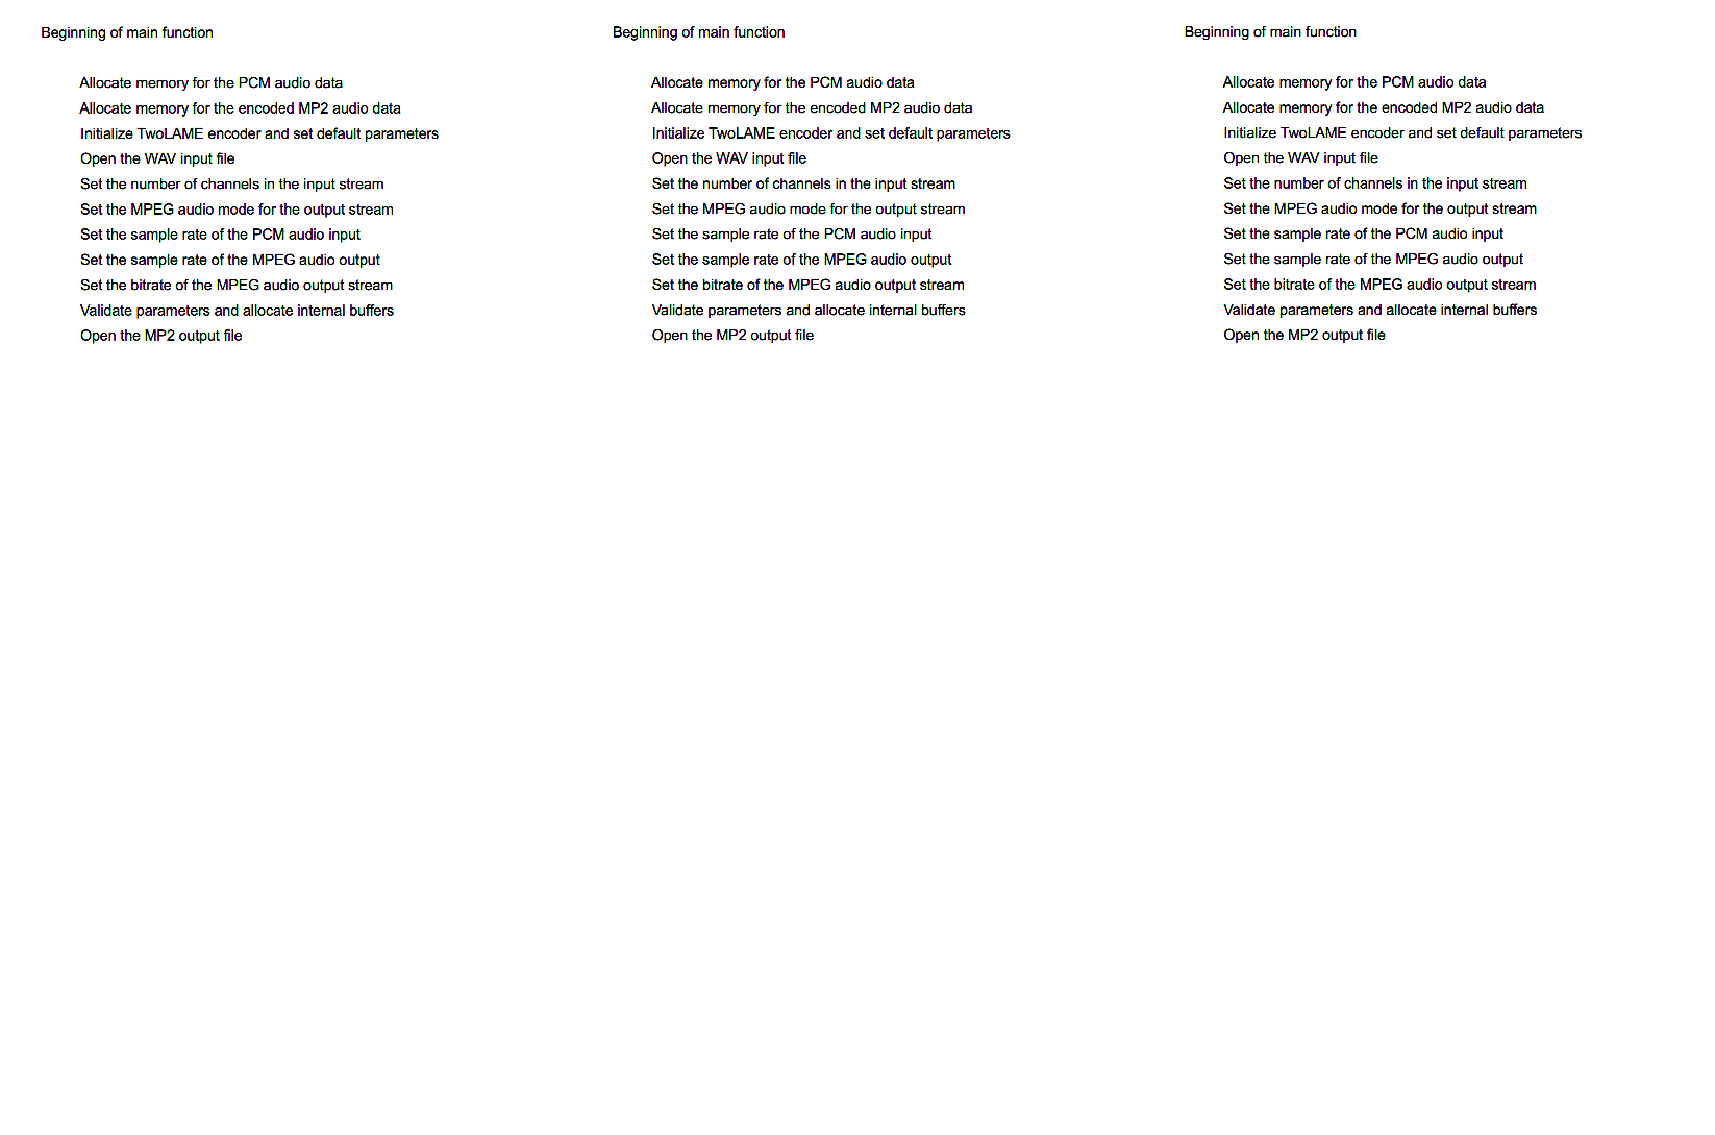
\includegraphics[width=0.80\linewidth]{pseudo1.pdf}}}
\caption{First part of \textit{firmware.c} pseudo code.}
\label{pseudo1}
\end{figure}

%\vspace{1cm}

The program starts by allocating memory for two different buffers to allow the encoding process. One of them is \textit{pcmaudio}, which receives part of the original input file. This PCM buffer has a size of AUDIOBUFSIZE multiplied by two (corresponds to the number of bytes of short integer type), being allocated and initialized with zero by \textit{calloc}. The other buffer is \textit{mp2buffer}, which receives part of the encoded file that is later written in the output file. This MP2 buffer has a size of MP2BUFSIZE (corresponds to the number of bytes of unsigned char type), being allocated and initialized with zero by \textit{calloc} as well.

Then comes the \textit{TwoLAME}-related stuff. The first function is \textit{twolame\_init}, which initializes the encoding software by setting defaults for all parameters and returning a pointer necessary to all future \textit{TwoLAME} calls. The second function is \textit{wave\_init}, which parses the wave header. This function belongs to \textit{audio\_wave.c} and is responsible for processing the wave header (the first four bytes). Apart from identifying the file as WAVE, the header gives relevant information like sample rate and audio mode, which is collected in a \textit{wave\_info\_t} struct.
The remaining initialization functions specify encoding options. There is the \textit{twolame\_set\_num\_channels}, which sets the number of channels in the input stream. There is also the \textit{twolame\_set\_mode}, which sets the MPEG Audio Mode (like mono or stereo) for the output stream. In addition, the \textit{twolame\_set\_in\_samplerate} sets the sample rate of the PCM audio input, while the \textit{twolame\_set\_out\_samplerate} sets the sample rate of the MPEG audio output. The \textit{twolame\_set\_bitrate} sets the bitrate of the MPEG audio output stream.

After defining the main encoding options, \textit{twolame\_init\_params} function is called. It prepares \textit{TwoLAME} to start encoding by checking all the parameters, making sure they are valid as well as allocating buffers and initializing internally used variables. Then, \textit{fopen} opens the output file where the encoded MP2 data is later written.

Moving to the \textit{TwoLAME} execution, figure \ref{pseudo2} shows the pseudo code for the second part of \textit{simplefrontend.c}, mainly consisting of the encoding process.

\begin{figure}[H]
\centerline{\fbox{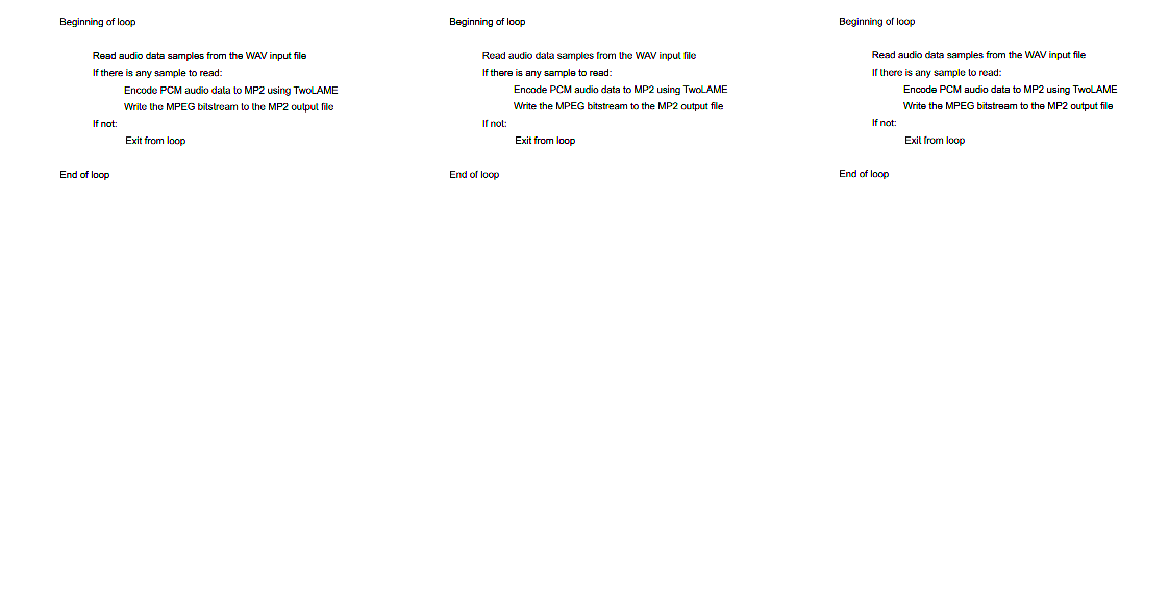
\includegraphics[width=0.80\linewidth]{pseudo2.pdf}}}
\caption{Second part of \textit{firmware.c} pseudo code.}
\label{pseudo2}
\end{figure}

%\vspace{1cm}

This process is based on a \textit{while} loop, as the main idea is to encode one part of the input audio file at a time, repeating the loop as many times as required. Therefore, each loop iteration starts by reading a chunk of audio data from the input WAV file through \textit{wave\_get\_samples}. This function also belongs to \textit{audio\_wave.c} and is responsible for reading AUDIOBUFSIZE samples to the PCM buffer (\textit{pcmaudio}).\\
With the buffer already loaded, \textit{twolame\_encode\_buffer\_interleaved} is responsible for encoding the audio data using TwoLAME. This function has a high level of complexity, as expected. It makes use of the \textit{libtwolame} library, which englobes many processes. In particular, the function is composed by \textit{twolame\_buffer\_init}, which sets the \textit{bit\_stream} struct, and \textit{encode\_frame}, which encodes one audio frame at a time.
After being encoded, the chunk of data is written in the output file through \textit{fwrite}. The \textit{frames} variable, which counts the number of frames encoded, is also updated. \\

Lastly, figure \ref{pseudo3} shows the pseudo code for the third part of \textit{simplefrontend.c}. 

\begin{figure}[H]
\centerline{\fbox{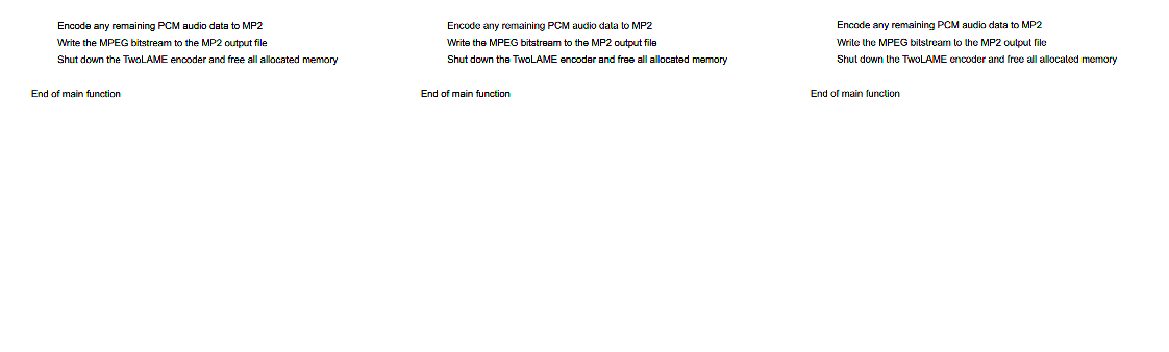
\includegraphics[width=0.80\linewidth]{pseudo3.pdf}}}
\caption{Third part of \textit{firmware.c} pseudo code.}
\label{pseudo3}
\end{figure}

%\vspace{1cm}

In this part, the \textit{TwoLAME} software finishes execution and so does the IOb-SoC system.
The first function is \textit{twolame\_encode\_flush}, which encodes any remaining buffered PCM audio, i.e., any remaining audio samples in the PCM buffer. This function is simpler than \textit{twolame\_encode\_buffer\_interleaved} and returns at most a single frame.
The \textit{fwrite} is used once again to write the remaining encoded data in the output file. Lastly, the encoding software is closed through \textit{twolame\_close} function. It shuts down the \textit{TwoLAME} encoder and frees all memory that was previously allocated, including PCM and MP2 buffers.

%%%%%%%%%%%%%%%%%%%%%%%%%%%%%%%%%%%%%%%%%%%%%%%%%%%%%%%%%%%%%%
    %current.tex below
%%%%%%%%%%%%%%%%%%%%%%%%%%%%%%%%%%%%%%%%%%%%%%%%%%%%%%%%%%%%%%

%Definição e proposta de metodologias a usar, com vista à consecução dos objetivos da Dissertação
%Resultados esperados e eventuais resultados preliminares

\subsection{System-on-Chip}
A System-on-Chip (SoC) is an integrated circuit that combines components of an electronic system. These components usually include a Central Processing Unit (CPU), memory interfaces, on-chip input/output devices, input/output interfaces, and secondary storage interfaces.\\
Putting many elements of a computer system on a single piece of silicon has some advantages, such as low power requirements, reduced cost, increased performance, and reduced physical size.

%iob-soc (%components, FPGA resources, repository, accelerators)
The IOb-SoC is a System-on-Chip template, comprising an open-source RISC-V processor, which users can modify, simulate, and implement in ASICs and FPGAs.
This SoC, provided by \textit{IObundle, Lda}, supports stand-alone and boot-loading modes. It also allows an internal RAM or an external DDR controller via an L1/L2 cache system. 

Figure \ref{fig:iob} shows the IOb-SoC high-level block diagram.

\vspace{0.1cm}

\begin{figure}[H]
\centerline{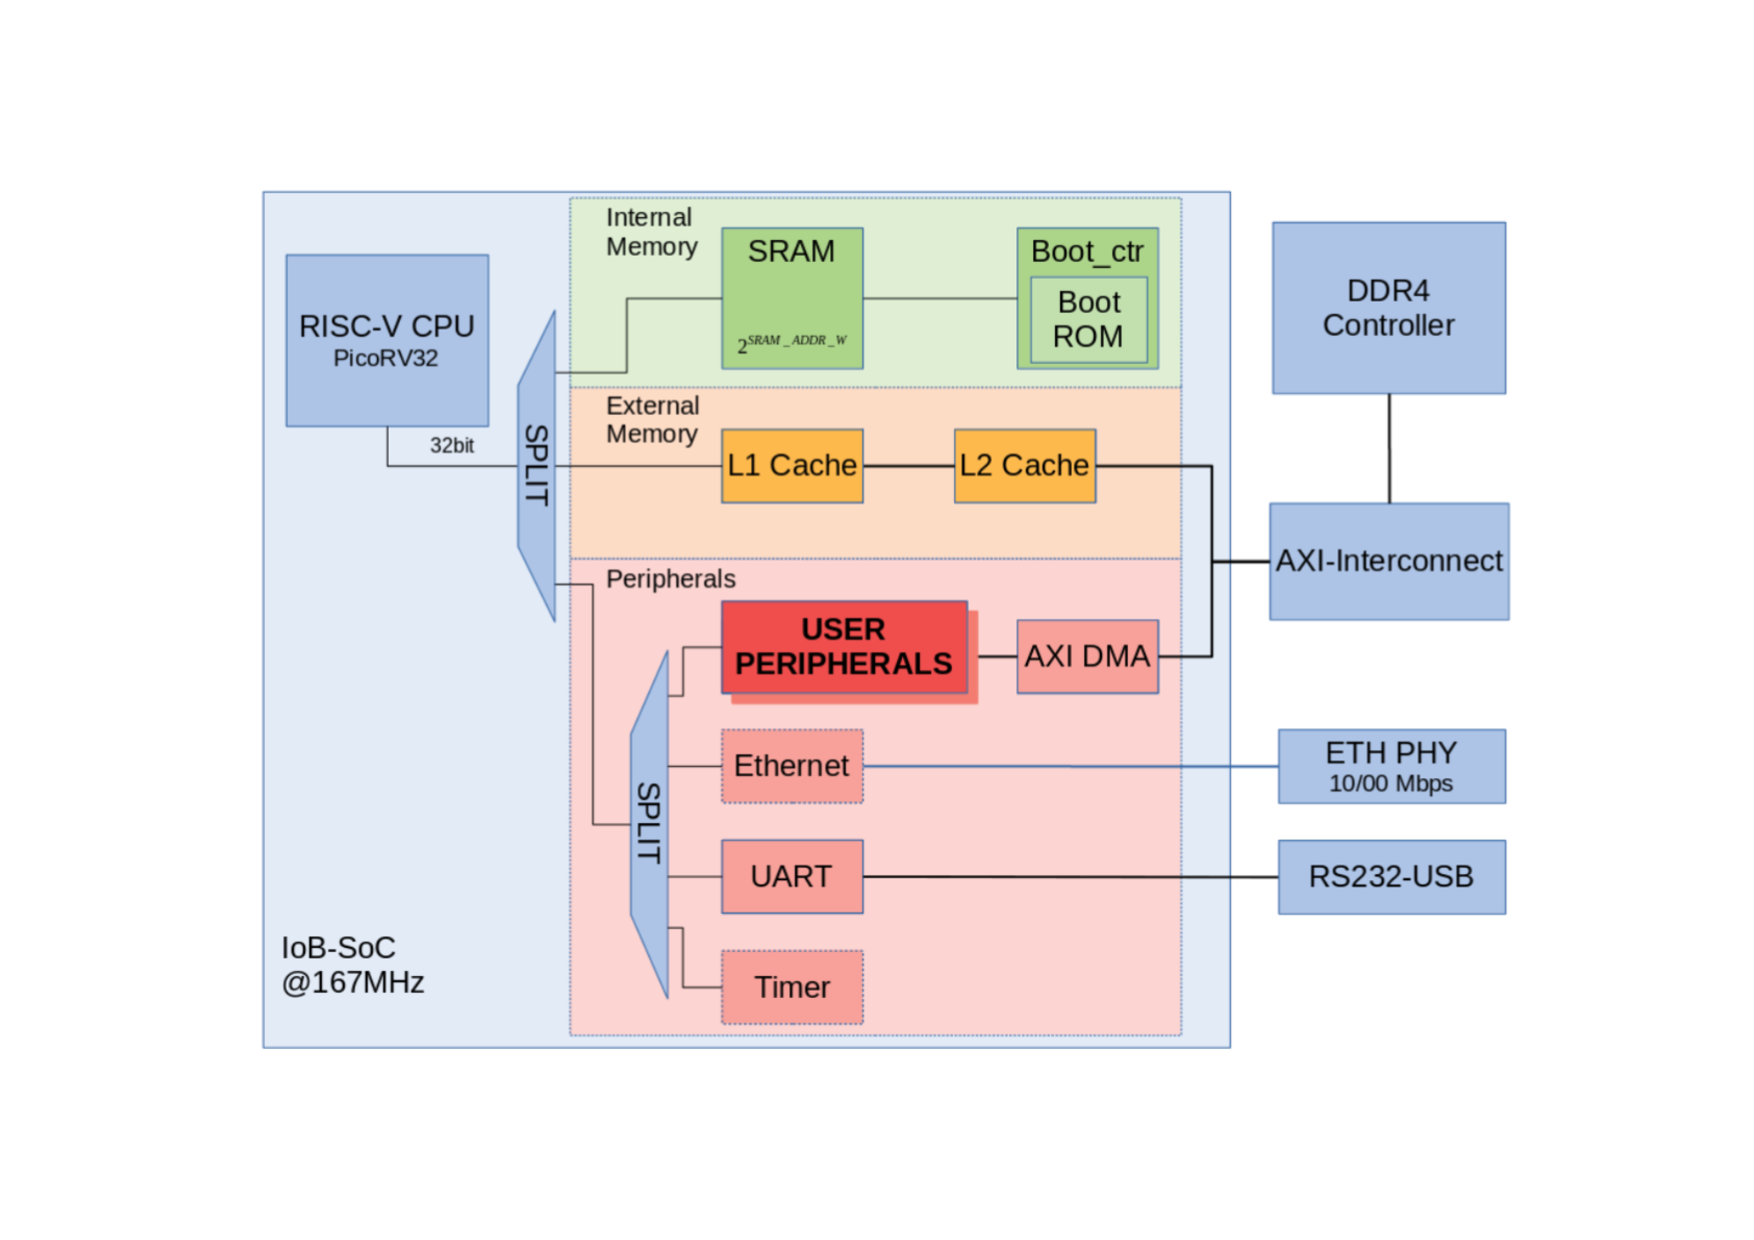
\includegraphics[width=0.85\linewidth]{iob-soc.pdf}}
\caption{IOb-SoC high-level block diagram.}
\label{fig:iob}
\end{figure}

\subsubsection{IOb-SoC Components}
Starting with the \textbf{CPU}, the IOb-SoC uses a PicoRV32 CPU core, an open-source 32-bit processor that implements the RV32IMC instruction set, with an operating frequency of 167MHz.

As \textbf{Memory} subsystem, this SoC includes three main components. The Boot Read-Only Memory \textbf{Boot ROM} is a ROM used for booting the system. The Static Random Access Memory \textbf{SRAM} is an internal memory that allows the system to run the program or the bootloader without the need for external memory. The \textbf{Cache} is an optional component that stores data from the external Double Data Rate (DDR) memory.

The communication between the CPU and the system’s components (master and slaves) occurs through two buses. The \textbf{Memory bus} allows the CPU to communicate with the memory subsystem, while the \textbf{Peripheral bus} allows the CPU to communicate with system peripherals.

In addition, the \textbf{IOb-Interconnect} component is a bus switch responsible for the valid-ready handshake protocol between the CPU and all the peripherals. Based on the peripheral prefix from the address bus, this component selects which peripheral-specific bus connects to the CPU bus. \\
The \textbf{IOb-Interconnect} multiplexes or demultiplexes, depending on the direction, the CPU bus signals (\textit{valid}, \textit{ready} and \textit{rdata}). By doing so, the component creates enough signals to ensure that there is one of each signal for each of the peripherals. Optionally, two peripherals connected to the peripheral bus can communicate directly without CPU intervention, allowing for faster data transfers between peripherals.

There is also a \textbf{Native to AXI adapter}, which allows communication between peripherals and memory controllers that use the AXI4 protocol. Since the CPU only contains the native bus, the IOb-SoC uses this component to convert the signals from one bus to the other, with each peripheral that uses the AXI4-Lite port containing one \textbf{Native to AXI adapter}.

Finally, The Universal Asynchronous Receiver-Transmitter (\textbf{\textbf{UART}}) peripheral allows the SoC to communicate with external systems, through the RS-232 serial communication protocol. \\

All these components are integrated into IOb-SoC as GitHub submodules. They belong to repositories tracked by GitHub and forked from \textit{IObundle, Lda}, but arranged in a different way and with specific names.
In this work, the IOb-SoC system comprises seven main components/submodules: \textbf{AXI}, an AXI interconnect protocol;
\textbf{CACHE}, a high-performance Verilog cache; \textbf{LIB}, a set of Verilog macros; \textbf{MEM}, a set of memory Verilog descriptions; \textbf{PICORV32}, a RISC-V processor; \textbf{TWOLAME}, an optimized MP2 encoding software; \textbf{UART}, a UART core. 

\subsubsection{IOb-SoC Deliverables and FPGA Resources}
As deliverables, the IOb-SoC includes Hardware Description Language (HDL) source code, software C source code, simulation testbench, implementation constraints for map, place, and route, demo files, and user documentation for system integration.

Tables~\ref{tab:resorucesxilinx} and~\ref{tab:resorucescyclone} show the implementation resources used for \textit{Xilinx Kintex Ultrascale Devices} and \textit{Intel Cyclone V Devices}, respectively, according to the product brief.

\vspace{0.8cm}

\begin{table}[H]
\parbox{.45\linewidth}{
\centering
\begin{tabular}{|c|c|c|}
        \hline
         \textbf{Resource} & \textbf{Usage}  \\
         \hline
         LUTs & 1869 \\
         \hline
         Registers & 1029 \\
         \hline
         DSPs & 4 \\
         \hline
         BRAM & 5 \\
         \hline
         PIN & 6 \\
         \hline
\end{tabular}
\caption{Implementation resources for Xilinx Kintex
Ultrascale Devices.}
\label{tab:resorucesxilinx}
}
\hfill
\parbox{.45\linewidth}{
\centering
\begin{tabular}{|c|c|c|}
        \hline
         \textbf{Resource} & \textbf{Usage}  \\
         \hline
         ALM & 1335 \\
         \hline
         FF & 1177 \\
         \hline
         DSP & 3 \\
         \hline
         BRAM blocks & 22 \\
         \hline
         BRAM bits & 165,888 \\
         \hline
         PIN & 6 \\
         \hline
\end{tabular}
\caption{Implementation resources for Intel Cyclone
V Devices.}
\label{tab:resorucescyclone}
}
\end{table}

%If the external memory interface is selected, an instruction L1 cache, a data L1 cache, and a shared L2 cache are added to the system. The L2 cache communicates with a 3rd party memory controller IP (typically a DDR controller) using an AXI4 master bus.

\subsubsection{IOb-SoC Repository}

%peripherals
%simulators and FPGA
The IOb-SoC Repository is a \textit{GitHub} repository that allows the user to modify the system components easily. It contains specific directories and segments (Tool Command Language (TCL), Verilog, Makefile, etc), with the list below describing the main items.

\textbf{document/} This directory supports all the documentation, from LaTeX code and scripts to generated PDFs, like the guide and product brief.

\textbf{hardware/} This directory supports the hardware layer, containing multiple subdirectories.

\hspace{0.5cm} – \textbf{hardware.mk} This makefile contains targets, dependencies, and rules related to hardware.

\hspace{0.5cm} – \textbf{fpga/} This directory contains scripts to synthesize and run the system in FPGAs.

\hspace{1.2cm}\textbf{fpga.mk} This makefile contains targets, dependencies, and rules related to FPGAs.

\hspace{0.5cm} – \textbf{simulation/} This directory contains scripts to run RTL simulation in simulators.

\hspace{1.2cm}\textbf{simulation.mk} This makefile contains targets, dependencies, and rules related to simulators.

\hspace{0.5cm}– \textbf{src/} This directory contains Verilog scripts related to the system’s components.

\textbf{software/} This directory supports the software layer, containing multiple subdirectories.

\hspace{0.5cm}– \textbf{software.mk} This makefile contains targets, dependencies, and rules related to software.

\hspace{0.5cm}– \textbf{firmware/} This directory contains the software to run in the system, after initialization.

\hspace{0.5cm}– \textbf{bootloader/} This directory contains the bootable software for the system.

\hspace{0.5cm}– \textbf{pc-emul/} This directory contains scripts to run the firmware on the computer.

\hspace{0.5cm}– \textbf{console/} This directory contains the software that allows interaction between computer and FPGA, via UART.

\textbf{submodules/} This directory contains all submodules and peripherals used in the system. While the peripherals are added to the peripheral bus, the submodules only represent components that are integrated into the system. 

\textbf{config.mk} This makefile contains targets, dependencies, and rules related to the SoC configuration, like the list of peripherals.

\subsection{ISO/SEC 11172-3: 1993 (E)}

The ISO/IEC 11172 is an international standard under the title \textit{Information technology - Coding of moving pictures and associated audio for digital storage media at up to about 1,5 Mbit/s}. This standard is divided into four parts (Systems, Video, Audio, and Compliance testing), with the Audio part being the relevant one for this work.

Focusing on the audio, the ISO/IEC 11172-3 specifies the coded representation of high-quality audio for storage media, and also the method for decoding high-quality audio signals. \\
Therefore, this part is intended for application to digital storage media. It provides a total continuous transfer rate of around 1.5Mbits/sec for both audio and video bitstreams, with sampling rates of 32kHz, 44.1kHz, and 48kHz.

\subsubsection{Audio encoder}

The audio encoder is responsible for processing the digital audio signal and producing the compressed bitstream for storage. 
The encoder algorithm is not standardized and may use various means of encoding, such as estimation of the auditory masking threshold, quantization, and scaling. However, the encoder output must be such that a decoder, conforming to the specifications of the coded audio bitstream, will produce audio suitable for the intended application.

%figure page v iso
Figure \ref{fig:encoder} illustrates the basic structure of an audio encoder. 

\begin{figure}[H]
\centerline{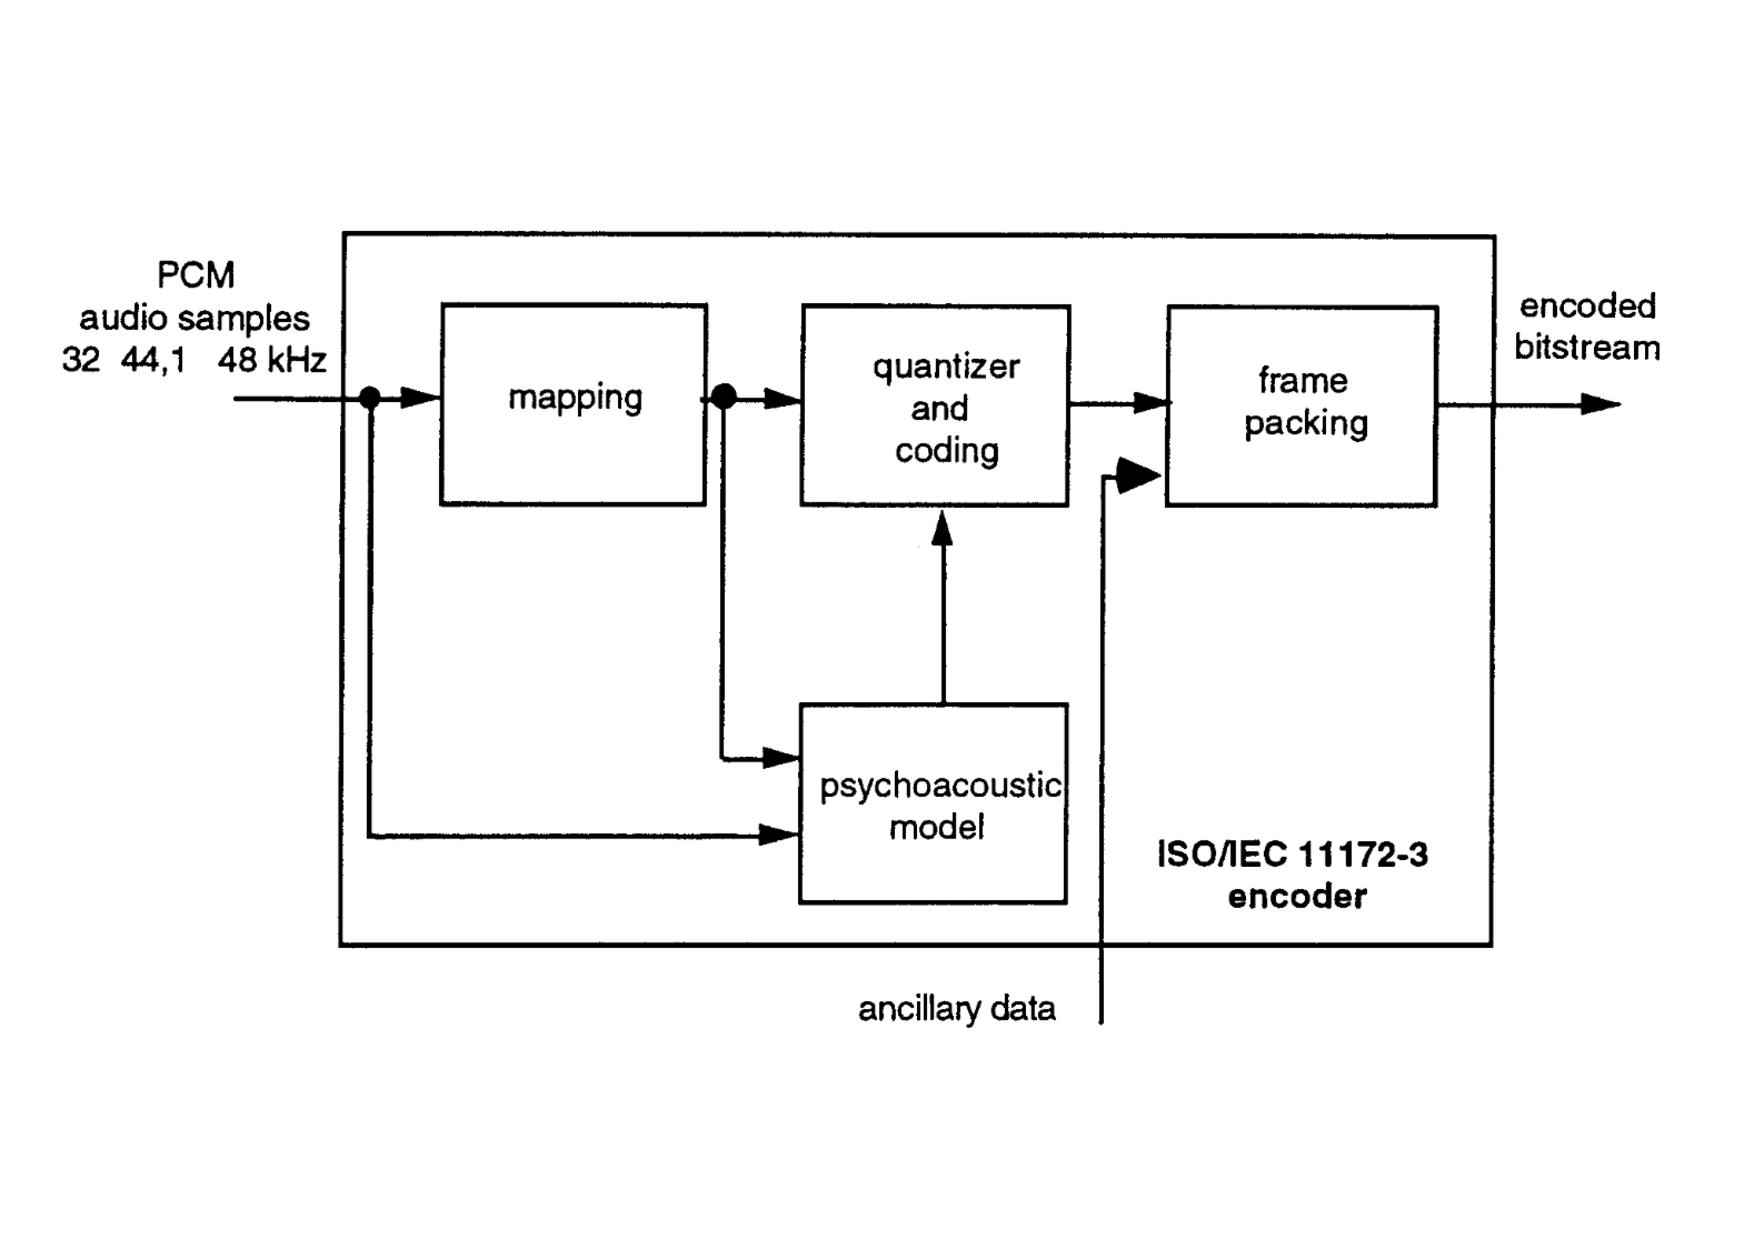
\includegraphics[width=0.85\linewidth]{encoder.pdf}}
\caption{Audio encoder basic structure.}
\label{fig:encoder}
\end{figure}

The encoding process contains four main blocks: \textit{mapping}, \textit{psychoacoustic model}, \textit{quantizer and coding}, and \textit{frame packing}.

First, the \textbf{mapping} block creates a filtered and subsampled representation of the input audio stream, usually called subband samples (for Layer II). At the same stage, the \textbf{psychoacoustic model} block creates a set of data to control the next block (\textit{quantizer and coding}). These control data depend on the coder implementation, with one possibility being the use of a masking threshold estimation.

Then, the \textbf{quantizer and coding} block creates a set of coding symbols from the mapped input samples, depending on the encoding system once again. 

Finally, the \textbf{frame packing} block assembles the actual bitstream from the output data of the previous blocks, adding information if necessary.

The encoding process supports four different modes: single channel, dual channel (two independent audio signals coded within one bitstream), stereo (left and right signals of a stereo pair coded within one bitstream), and Joint Stereo (with the stereo irrelevancy and redundancy exploited).

\subsubsection{Psychoacoustic encoder}

The ISO/IEC 11172-3 (MPEG-Audio) psychoacoustic algorithm contains four primary parts, as shown in figure \ref{fig:algorithm}: \textit{Filter Bank}, \textit{Psychoacoustic Model}, \textit{Bit or Noise Allocation} and \textit{Bitstream Formatting}.

%figure page 66 iso
\begin{figure}[H]
\centerline{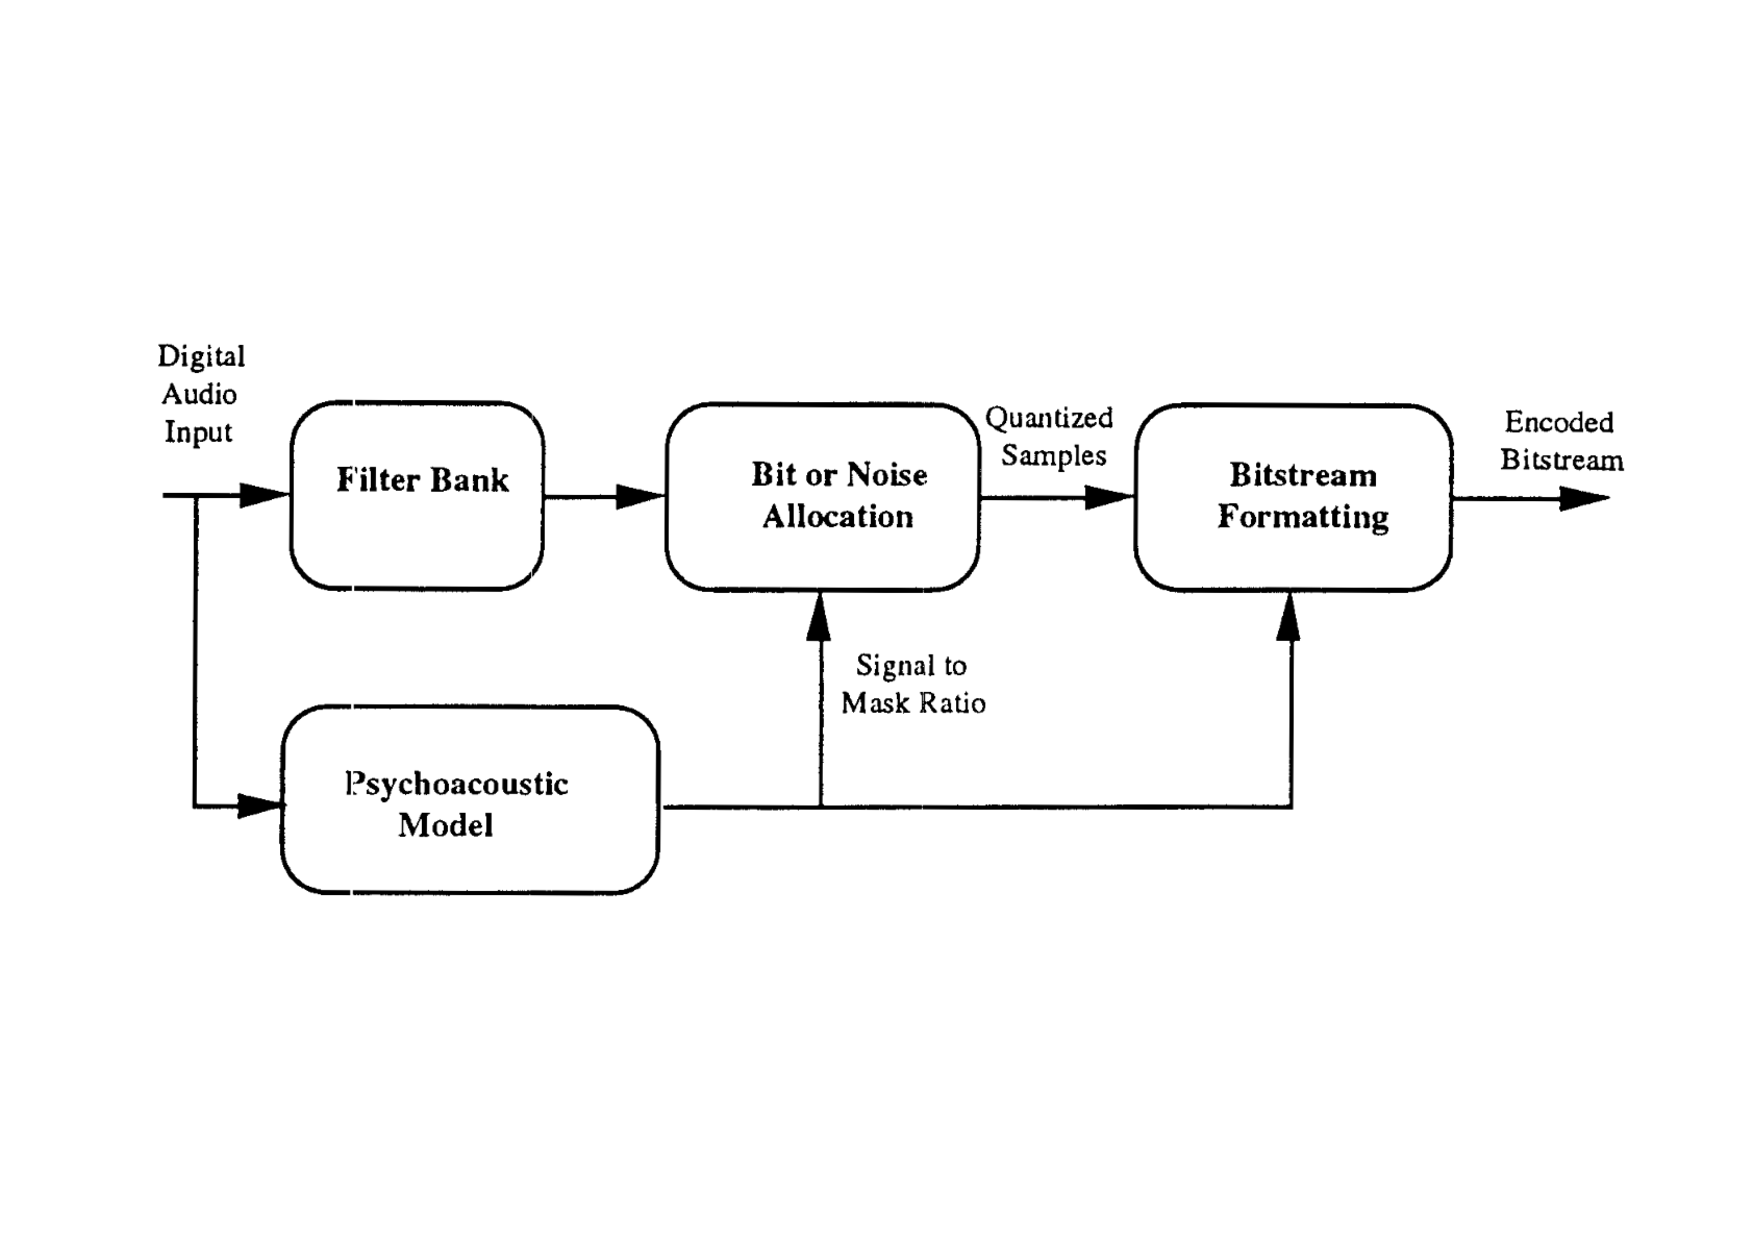
\includegraphics[width=0.85\linewidth]{iso-encoder.pdf}}
\caption{ISO/IEC 11172-3 encoder block diagram.}
\label{fig:algorithm}
\end{figure}

The \textbf{Filter Bank} does a time-to-frequency mapping, being one of two types. It can be a polyphase filter bank or a hybrid polyphase/MDCT filter bank, with each delivering a specific mapping in time and frequency.
These filterbanks are critically sampled, having the same number of samples in both analyzed and time domains, and provide the primary frequency separation for the encoder, with quantized output samples. \\
In layer II, a filter bank with 32 subbands is used. In each subband, 12 or 36 samples are grouped for processing.

The \textbf{Psychoacoustic Model} calculates a just noticeable noise level for each band in the filter bank. This noise level is used in the \textit{Bit or Noise Allocation} part to determine the actual quantizers and quantizer levels. 
The final output of the model is a signal-to-mask ratio (SMR) for each band (Layer II).
%annex D  (MOdel 1 Layer II)

The \textbf{Bit or Noise Allocation} takes both the output samples from the \textit{Filter Bank} and the SMR from the \textit{Psychoacoustic Model} and adjusts the bit allocation, to meet the bitrate and masking requirements. At low bitrates, these methods attempt to spend bits in a way that is inoffensive when they cannot meet the psychoacoustic demand at the required bitrate.\\
In Layer II, this method is a bit allocation process, where several bits are assigned to each sample (or group of samples) in each subband.

The \textbf{Bitstream Formatting} takes the quantized filterbank outputs, together with the bit allocation and other required side information, and encodes and efficiently formats all that information.\\
In Layer II, a fixed Pulse code modulation (PCM) code is used for each subband sample, with the exception that quantized samples may be grouped.

%figure page 79 iso
Figure \ref{fig:flow-encoder} shows a more detailed Layer II Encoder flow chart.

\begin{figure}[H]
\centerline{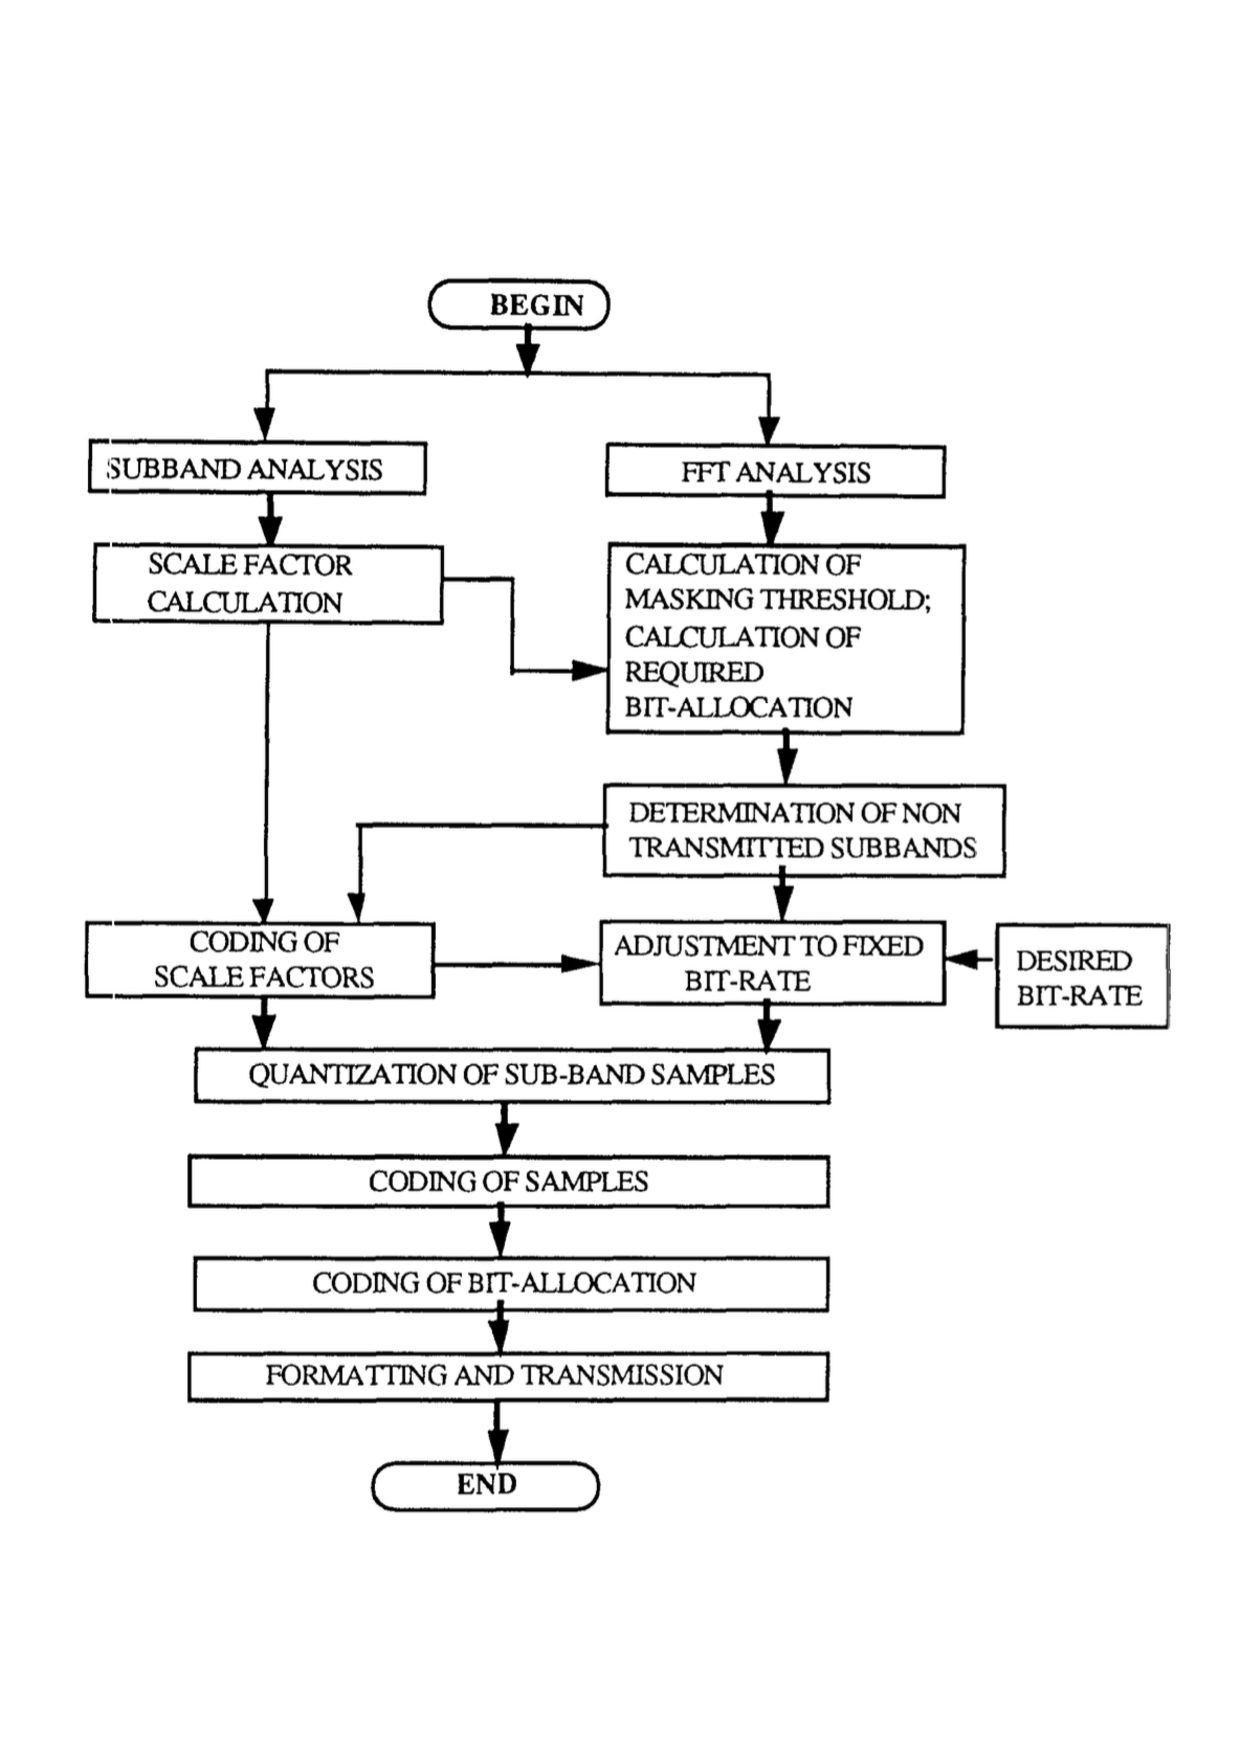
\includegraphics[width=0.70\linewidth]{flow-encoder.pdf}}
\caption{Layer II encoder flow chart.}
\label{fig:flow-encoder}
\end{figure}


\subsection{\textit{Versat}}

\textit{Versat} constitutes a reconfigurable hardware accelerator tailored for integration within embedded systems. Operating on a Coarse-Grain Reconfigurable Array (CGRA) architecture, \textit{Versat} exhibits compact dimensions and low power consumption. The design features a simplified controller unit, facilitating self and partial reconfiguration.

The architecture is characterized by a modest number of functional units interlinked in a comprehensive graph topology to ensure optimal adaptability. The reduced functional unit count is offset by the ease of configuration and dynamic reconfiguration during runtime. Distinguishing itself from conventional CGRAs, \textit{Versat} is proficient in mapping sequences of nested program loops rather than individual loops, with self and partial reconfiguration occurring between these nested loops.

Programming \textit{Versat} is achievable through assembly language and a specialized C++ dialect. The ability to program using assembly language presents a novel and valuable aspect for program optimization and circumventing compiler or architectural challenges.
Regarding practical utilization, \textit{Versat} can serve as an accelerator for host processors on the same chip, enabling certain procedures to run faster and consume less energy when executed on \textit{Versat}. To diminish dependency on the host Central Processing Unit (CPU), \textit{Versat} incorporates a straightforward Controller responsible for algorithmic control, self-reconfiguration, and data movement. This frees up the host for more productive tasks. The Controller is programmable and encompasses an instruction memory storing \textit{Versat} programs. Control over the various modules is administered through a Control Bus.

Incorporated within \textit{Versat} is a dedicated Data Engine (DE) unit that conducts data computation. The DE unit comprises Functional Units (FUs) interconnected in a complete mesh, offering multiple configurations for a given datapath. This multiplicity aids in simplifying the compiler.
The Configuration Module (CM) retains the DE's configuration, specifying the present datapath, and accommodates a register for preparing the subsequent configuration of the DE. Additionally, it possesses another register capable of temporarily storing numerous complete configurations, switchable during runtime. The Controller can write partial configurations to the CM and manage to save and restore entire configurations from the configuration memory.

Furthermore, \textit{Versat} integrates a Direct Memory Access (DMA) module, enabling autonomous and efficient data, program, and configuration transfers in and out of the device. The DMA operates through a master Advanced Extensible Interface – AXI4, an interface stemming from the Advanced Microcontroller Bus Architecture (AMBA) and designed by ARM.

Facilitating communication with the host processor, \textit{Versat} is equipped with a shared Control Register File (CRF). The CRF incorporates two host interfaces, selectable during compilation: a Serial Peripheral Interface (SPI) and a parallel bus interface. The SPI slave interface is employed when the host system is an off-chip master device, primarily for debugging and testing purposes. On the other hand, the parallel bus interface is utilized when the host is an embedded processor and may adhere to the AXI4 Lite format.

\textit{Versat} is compatible with IOb-Soc. It can be integrated as a peripheral, since it contains an internal AXI DMA that communicates with IOb-SoC's memory system, through an AXI-Interconnect. Figure \ref{fig:iobversat} shows the high-level block diagram of \textit{Versat} integrated into IOb-SoC.

\vspace{0.1cm}

\begin{figure}[H]
\centerline{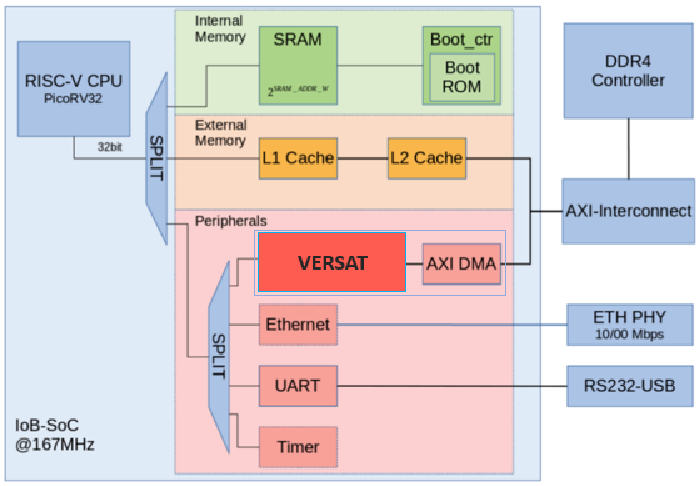
\includegraphics[width=0.85\linewidth]{iob-soc-versat.pdf}}
\caption{\textit{Versat} integrated in IOb-SoC high-level block diagram.}
\label{fig:iobversat}
\end{figure}

\subsubsection{Functional units}
In practical terms, \textit{Versat} is a reconfigurable hardware accelerator that contains several functional units (FUs) in its source, all written in Verilog. Nonetheless, the user has the possibility of creating and adding new ones to the source.


A brief description of each functional unit is provided in the table below.

\begin{table}[H]
    \centering
    \begin{tabular}{|c|p{0.8\linewidth}|}
        \hline
        \multicolumn{1}{|c|}{\textbf{FU}} & \multicolumn{1}{c|}{\textbf{Description}} \\
        \hline
        \multirow{1}{*}{\textit{Const}} & This module receives a 32-bit input and outputs the same 32-bit value.  \\
        \hline
        \multirow{2}{*}{\textit{FloatAdd}} & This module receives two 32-bit floating-point inputs, adds them together, and outputs a 32-bit floating-point value. \\
        \hline
        \multirow{2}{*}{\textit{FloatSub}} & This module receives two 32-bit floating-point inputs, subtracts one from the other, and outputs a 32-bit floating-point value. \\
        \hline
        \multirow{2}{*}{\textit{FloatMul}} & This module receives two 32-bit floating-point inputs, multiplies them together, and outputs a 32-bit floating-point value. \\
        \hline
        \multirow{2}{*}{\textit{FloatNot}} & This module receives a 32-bit floating-point input, negates the most significant bit (MSB), and outputs a 32-bit floating-point value. \\
        \hline
        \multirow{6}{*}{\textit{Float2Int}} &  
        This module receives a 32-bit floating-point input and converts it to a 32-bit integer output. 
        It performs a conversion operation that truncates the fractional part of the floating-point input, effectively extracting the integer component. 
        The resulting 32-bit integer output represents the integer part of the input floating-point number. 
        In cases where the input is negative, the output will represent the floor of the absolute value of the input. \\
        \hline
        \multirow{4}{*}{\textit{Mux2}} & This module receives two 32-bit inputs and one 1-bit control input. 
        It operates as a 2-to-1 multiplexer, selecting one of the 32-bit inputs based on the 1-bit control input. 
        If the control input is zero, the output will be the first 32-bit input; otherwise, the output will be the second 32-bit input. \\
        \hline
        \multirow{7}{*}{\textit{Mem}} & This module contains an internal memory with two input and two output ports (True dual-port synchronous RAM). 
        It offers a memory-mapped interface that allows the CPU to store and read data from the memory while the \textit{Versat} accelerator is not running. 
        Internally, this module contains two Address Generator Units (AGU) that generate the addresses used to access the memory, one for each port. 
        The AGUs can be configured to output or store data (only one type per port, the same port cannot be configured to output and store data at the same time in one run). \\
        \hline
        \multirow{5}{*}{\textit{LookupTable}} & This module contains an internal memory with two input and two output ports (Dual port synchronous RAM). 
        It offers a memory-mapped interface that allows the CPU to store and read data from the memory while the \textit{Versat} accelerator is not running. 
        Internally, this module acts like a lookup table since the output is the value stored in the address given by the input. \\
        \hline
    \end{tabular}
    \caption{Table of functional units.}
    \label{tab:fu}
    \end{table}
    
\vspace{0.5cm}

\subsubsection{Operators}

\textit{Versat} also contains a set of 6 operators defined in its specification source. The operators execute either over the right operand or between the left and right operands.

A brief description of each operator is provided in the table below.

\begin{table}[H]
    \centering
    \begin{tabular}{|c|p{0.8\linewidth}|}
        \hline
        \multicolumn{1}{|c|}{\textbf{Operator}} & \multicolumn{1}{c|}{\textbf{Description}} \\
        \hline
        \multirow{1}{*}{\textbf{$-$}} & This operator negates the right operand.  \\
        \hline
        \multirow{1}{*}{\textbf{$\sim$}} & This operator negates the MSB of the right operand. \\
        \hline
        \multirow{1}{*}{\textbf{$\And$}} & This operator performs a logical AND between the left and right operands. \\
        \hline
        \multirow{2}{*}{\textbf{$\ll$}} & This operator shifts the bits of the left operand to the left by the number of positions defined by the right operand. \\
        \hline
        \multirow{1}{*}{\textbf{$\vert$}} & This operator performs a logical OR between the left and right operands. \\
        \hline
        \multirow{1}{*}{\textbf{$\wedge$}} & This operator performs a logical XOR between the left and right operands. \\
        \hline
    \end{tabular}
    \caption{Table of operators.}
    \label{tab:op}
\end{table}

\vspace{0.5cm}

\subsubsection{Syntax}

Knowing the FUs and operators \textit{Versat} provides, it is convenient to understand how the hardware design can be developed using such resources.
Figure \ref{versatspec} shows a coding example of \textit{versatSpec.txt}, the file where the \textit{Versat} accelerator should be described.

\vspace{1cm}

\begin{figure}[H]
\centerline{\fbox{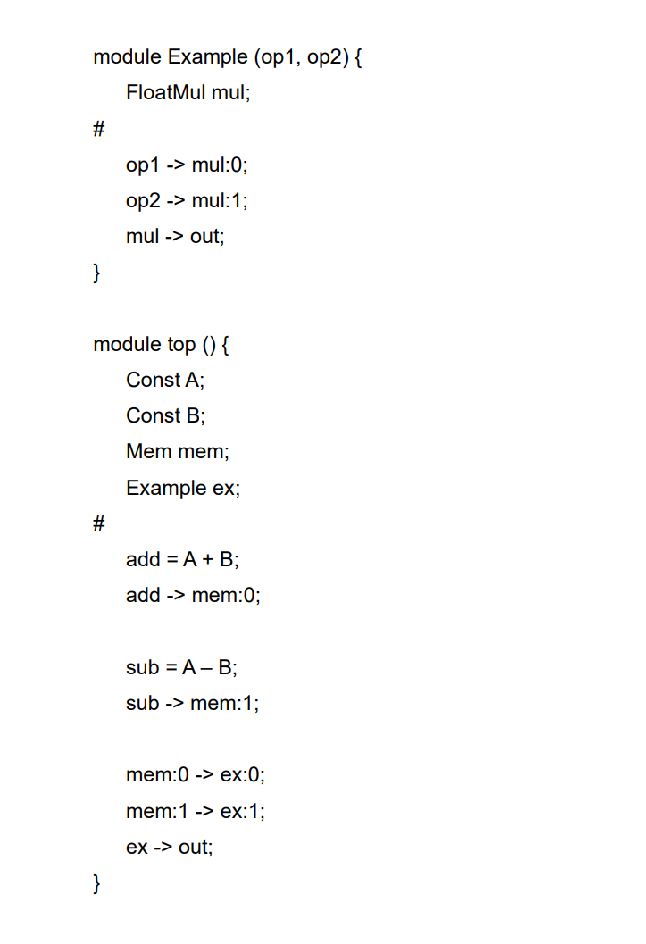
\includegraphics[width=0.60\linewidth]{versatspec.pdf}}}
\caption{\textit{versatspec.txt} example.}
\label{versatspec}
\end{figure}

Focusing on the syntax, the code is divided into two modules, \textit{Example} and \textit{top}, each representing a part of the hardware design.

The \textit{Example} module is defined with two input ports, \textit{op1} and \textit{op2}, and a \textit{FloatMul} FU, \textit{mul}. 
The code after the \# symbol specifies how data flows through the module. In this case, \textit{op1} and \textit{op2} are connected to input ports 0 and 1 of the \textit{mul} FU, respectively. \\
Then, the output of the \textit{mul} FU is connected to the output port of the \textit{Example} module.

The \textit{top} module is the starting module, i.e. it represents the overall design.
This module is defined with two \textit{Const} FUs, \textit{A} and \textit{B}, and a \textit{Mem} FU, \textit{mem}. In addition, it also contains an instance of the \textit{Example} module called \textit{ex}.\\
Once again, the code specifies how data flows through the modules. In this case, \textit{A} and \textit{B} are added together, and the result is stored in the \textit{add} signal. Then, \textit{add} is connected to input port 0 of the \textit{mem} FU.\\
\textit{A} and \textit{B} are also subtracted, and the result is stored in the \textit{sub} signal. Then, \textit{sub} is connected to input port 1 of the \textit{mem} FU.
Afterward, the output ports 0 and 1 of \textit{mem} are connected to the input ports 0 and 1 of \textit{ex} instance, respectively. 
The \textit{ex} instance performs what was described previously for the \textit{Example} module, and its output is connected to the output port of the top module.

In terms of functionality, this example starts by performing arithmetic operations on constants \textit{A} and \textit{B}. Then, it sends the results of those operations to a memory unit, which works as indices for each data array (in each input port). Based on these indices, the memory unit outputs one value in each output port, which is then used in the following module to perform a floating-point multiplication operation. The final result is accessible through the output port of the top module.